% first example chapter
% @author Thomas Lehmann
%
\chapter{Konzeption des Systems}
Dieses Kapitel beschreibt die Konzeption des zu entwickelnden Systems. Zunächst 
werden Anforderungen und zentrale Use Cases definiert. Anschließend wird die 
Zielarchitektur und Systemübersicht erläutert, gefolgt vom Datenmodell und 
den Datenflüssen. Darauf aufbauend folgt die detaillierte Beschreibung der 
Prozessabläufe „Rechnung neu erstellen" und „Dokument ablegen". Abschließend 
wird das Sicherheits- und Datenschutzkonzept vorgestellt.

\section{Anforderungen und Use Cases}
Die Situation und das Problem, das damit verbunden ist, sind wie folgt:

Das geplante System richtet sich vor allem an kleine Dienstleistungsfirmen, Einzelunternehmer sowie kleine und mittlere Gewerbebetriebe. Diese müssen regelmäßig Rechnungen erstellen und verwalten, verfügen jedoch weder über die Ressourcen noch über den Bedarf für umfassende Buchhaltungs- oder \glspl{ac:erp}-Systeme. Häufig mangelt es diesen Personen an IT-Kenntnissen und sie haben wenig Zeit. Deshalb benötigen sie einfache, zuverlässige und größtenteils automatisierte Prozesse. Auch Steuerberaterinnen und Steuerberater sind auf vollständig und strukturiert archivierte Rechnungsunterlagen angewiesen. Studien und Praxisanalysen zeigen, dass manuelle Rechnungsprozesse in kleinen Unternehmen mit einem erhöhten Zeitaufwand, einer höheren Fehleranfälligkeit sowie häufigen Medienbrüchen verbunden sind, was zu einem Mangel an Transparenz in den Abrechnungsprozessen führen kann \cite{bitkom_elektronische_rechnungsdaten_2022,beckit_rechnungsverarbeitung_2022,pleo_automatisierte_rechnungsverarbeitung_2024}.

In der Praxis erfolgt die Erstellung von Rechnungen und Dokumenten in vielen dieser Unternehmen überwiegend manuell. Die Ablage geschieht häufig in unsystematischen Ordnerstrukturen. Dieser Ansatz ist zeitaufwendig und anfällig für Fehler, da Kundendaten und Rechnungspositionen wiederholt neu eingegeben werden müssen. Dadurch steigt das Risiko von Zahlendrehern, unvollständigen Daten oder fehlerhaften Summenberechnungen. Zudem erschwert eine unstrukturierte Ablage das spätere Wiederfinden einzelner Dokumente, insbesondere wenn Belege zu einem späteren Zeitpunkt für buchhalterische oder steuerliche Zwecke benötigt werden.

Rechnungen, die Fehler aufweisen oder verspätet erstellt werden, können den Zahlungseingang verzögern und damit die Liquidität der Unternehmen beeinträchtigen. Sind Dokumente unvollständig, unsortiert oder schwer auffindbar, verlängert sich nicht nur die Bearbeitungszeit von Kundenanfragen – was den professionellen Außenauftritt beeinträchtigen kann –, sondern auch der Aufwand, wenn Belege kurzfristig benötigt werden. Die nachträgliche Aufbereitung und Abstimmung solcher Unterlagen kostet zusätzliche Zeit und Ressourcen und erhöht das Risiko, dass steuerliche Erklärungen fehlerhaft oder verspätet eingereicht werden.

Ziele und Anforderungen aus Sicht der Anwender

Die Entlastung im täglichen Verwaltungs- und Abrechnungsalltag steht aus Anwendersicht im Vordergrund.  Das Ziel ist es, die Zeit und den Aufwand, die für die Erstellung und Verwaltung von Rechnungen benötigt werden, deutlich zu reduzieren, damit mehr Zeit für das eigentliche Kerngeschäft bleibt.

 Gleichzeitig besteht das Bedürfnis nach einer übersichtlichen und verlässlichen Ablage für geschäftsrelevante Dokumente.  Um Fehler zu vermeiden und die Effizienz der Arbeitsabläufe zu verbessern, ist es entscheidend, dass alle Daten vollständig, korrekt und einheitlich erfasst werden.

 Außerdem ist die Zusammenarbeit mit externen Partnern, vor allem mit Steuerberaterinnen und Steuerberatern, von großer Bedeutung.  Anwender gehen davon aus, dass alle benötigten Unterlagen aktuell, vollständig und gut strukturiert sind, um Rückfragen zu minimieren und zusätzlichen Abstimmungsaufwand zu vermeiden. 

Diese Ziele resultieren in konkreten funktionalen Anforderungen an das System. Es muss den Nutzern ermöglichen, bestehende Kundendaten auszuwählen oder neue Kundendatensätze mit allen relevanten Stammdaten anzulegen. Darüber hinaus soll das System alle für die Rechnungserstellung erforderlichen Informationen erfassen. Dazu zählen unter anderem Leistungsbeschreibungen, Mengenangaben, Einzelpreise, Steuersätze und Zahlungsfristen, die strukturiert und nachvollziehbar eingegeben werden können.

Nach Abschluss der Datenerfassung stellt das System das erstellte Rechnungsdokument bereit und ermöglicht zudem die Ablage weiterer geschäftsrelevanter Dokumente, sodass diese später erneut abgerufen werden können.


Nicht nur die funktionalen, sondern auch die nicht-funktionalen Anforderungen sind von großer Bedeutung. Um auch Menschen ohne technische Vorkenntnisse zu erreichen, soll das System benutzerfreundlich gestaltet sein, sodass der Prozess der Rechnungserstellung und -verwaltung intuitiv durchlaufen werden kann. Eine positive Nutzungserfahrung setzt zudem kurze Reaktionszeiten voraus, um lange Wartezeiten für die Nutzer zu vermeiden.

Darüber hinaus ist es wichtig, dass das Erstellen neuer Rechnungen sowie das Ablegen von Dokumenten zügig erfolgt, damit erzeugte oder hochgeladene Dateien ohne spürbare Verzögerung zur Verfügung stehen. Das System muss außerdem zuverlässig und fehlertolerant arbeiten. Eingabefehler sollen durch geeignete Validierungen erkannt und abgefangen werden, während die Abläufe stabil und reproduzierbar ausgeführt werden.

Da personenbezogene Daten und Abrechnungsinformationen verarbeitet werden, kommt der Datensicherheit eine besondere Bedeutung zu. Zugangsdaten sind sicher zu speichern, die Kommunikation ist zu verschlüsseln und der Zugriff auf autorisierte Nutzer zu beschränken. Weiterhin soll die Systemarchitektur modular und erweiterbar gestaltet sein, um zukünftige Anforderungen oder zusätzliche Funktionen mit vertretbarem Aufwand integrieren zu können. Insgesamt orientiert sich das System damit an anerkannten Qualitätsmerkmalen nicht-funktionaler Anforderungen, wie sie im Qualitätsmodell der ISO/IEC 25010 sowie in der Fachliteratur beschrieben sind \cite{iso_25010_2023,seibert_nfa_2018,johann_nfa_2025}.


Anwendungsfall „Rechnung neu erstellen“

Der Anwendungsfall „Rechnung neu erstellen“ beginnt, sobald der Nutzer die entsprechende Aktion auswählt und den Erstellungsprozess startet. Zunächst entscheidet der Nutzer, ob die Daten eines bestehenden Kunden verwendet oder ein neuer Kundendatensatz angelegt werden soll. Bei der Neuanlage werden alle erforderlichen Stammdaten wie Name oder Firmenbezeichnung, Adresse, Kontaktinformationen und gegebenenfalls steuerliche Angaben erfasst.

Im nächsten Schritt gibt der Nutzer die zu fakturierenden Leistungen an. Dazu zählen die Leistungsbeschreibung sowie die zugehörigen Mengen, Einzelpreise und gegebenenfalls anwendbare Steuersätze. Der Nutzer kann mehrere Rechnungspositionen nacheinander erfassen, sofern dies erforderlich ist.

Anschließend werden rechnungsbezogene Angaben wie Rechnungsnummer, Rechnungsdatum, Leistungszeitraum und Zahlungsfrist festgelegt. Nach Abschluss der Dateneingabe wird die Rechnung erstellt und dem Nutzer zur Verfügung gestellt.



Anwendungsfall „Dokument ablegen“
Der Anwendungsfall „Dokument ablegen“ beginnt, sobald der Nutzer die entsprechende Aktion auswählt, um geschäftsrelevante Dokumente im System zu archivieren. Hierzu lädt der Nutzer eine Datei, beispielsweise einen Beleg oder eine Rechnung, hoch.

Das System ordnet das Dokument dem entsprechenden Kunden zu und legt es strukturiert ab, sodass es später zuverlässig wiedergefunden werden kann. Nach dem Abschluss des Vorgangs steht das abgelegte Dokument dem Nutzer zur Einsicht und zum erneuten Abruf zur Verfügung.
\begin{figure}[H]
\centering
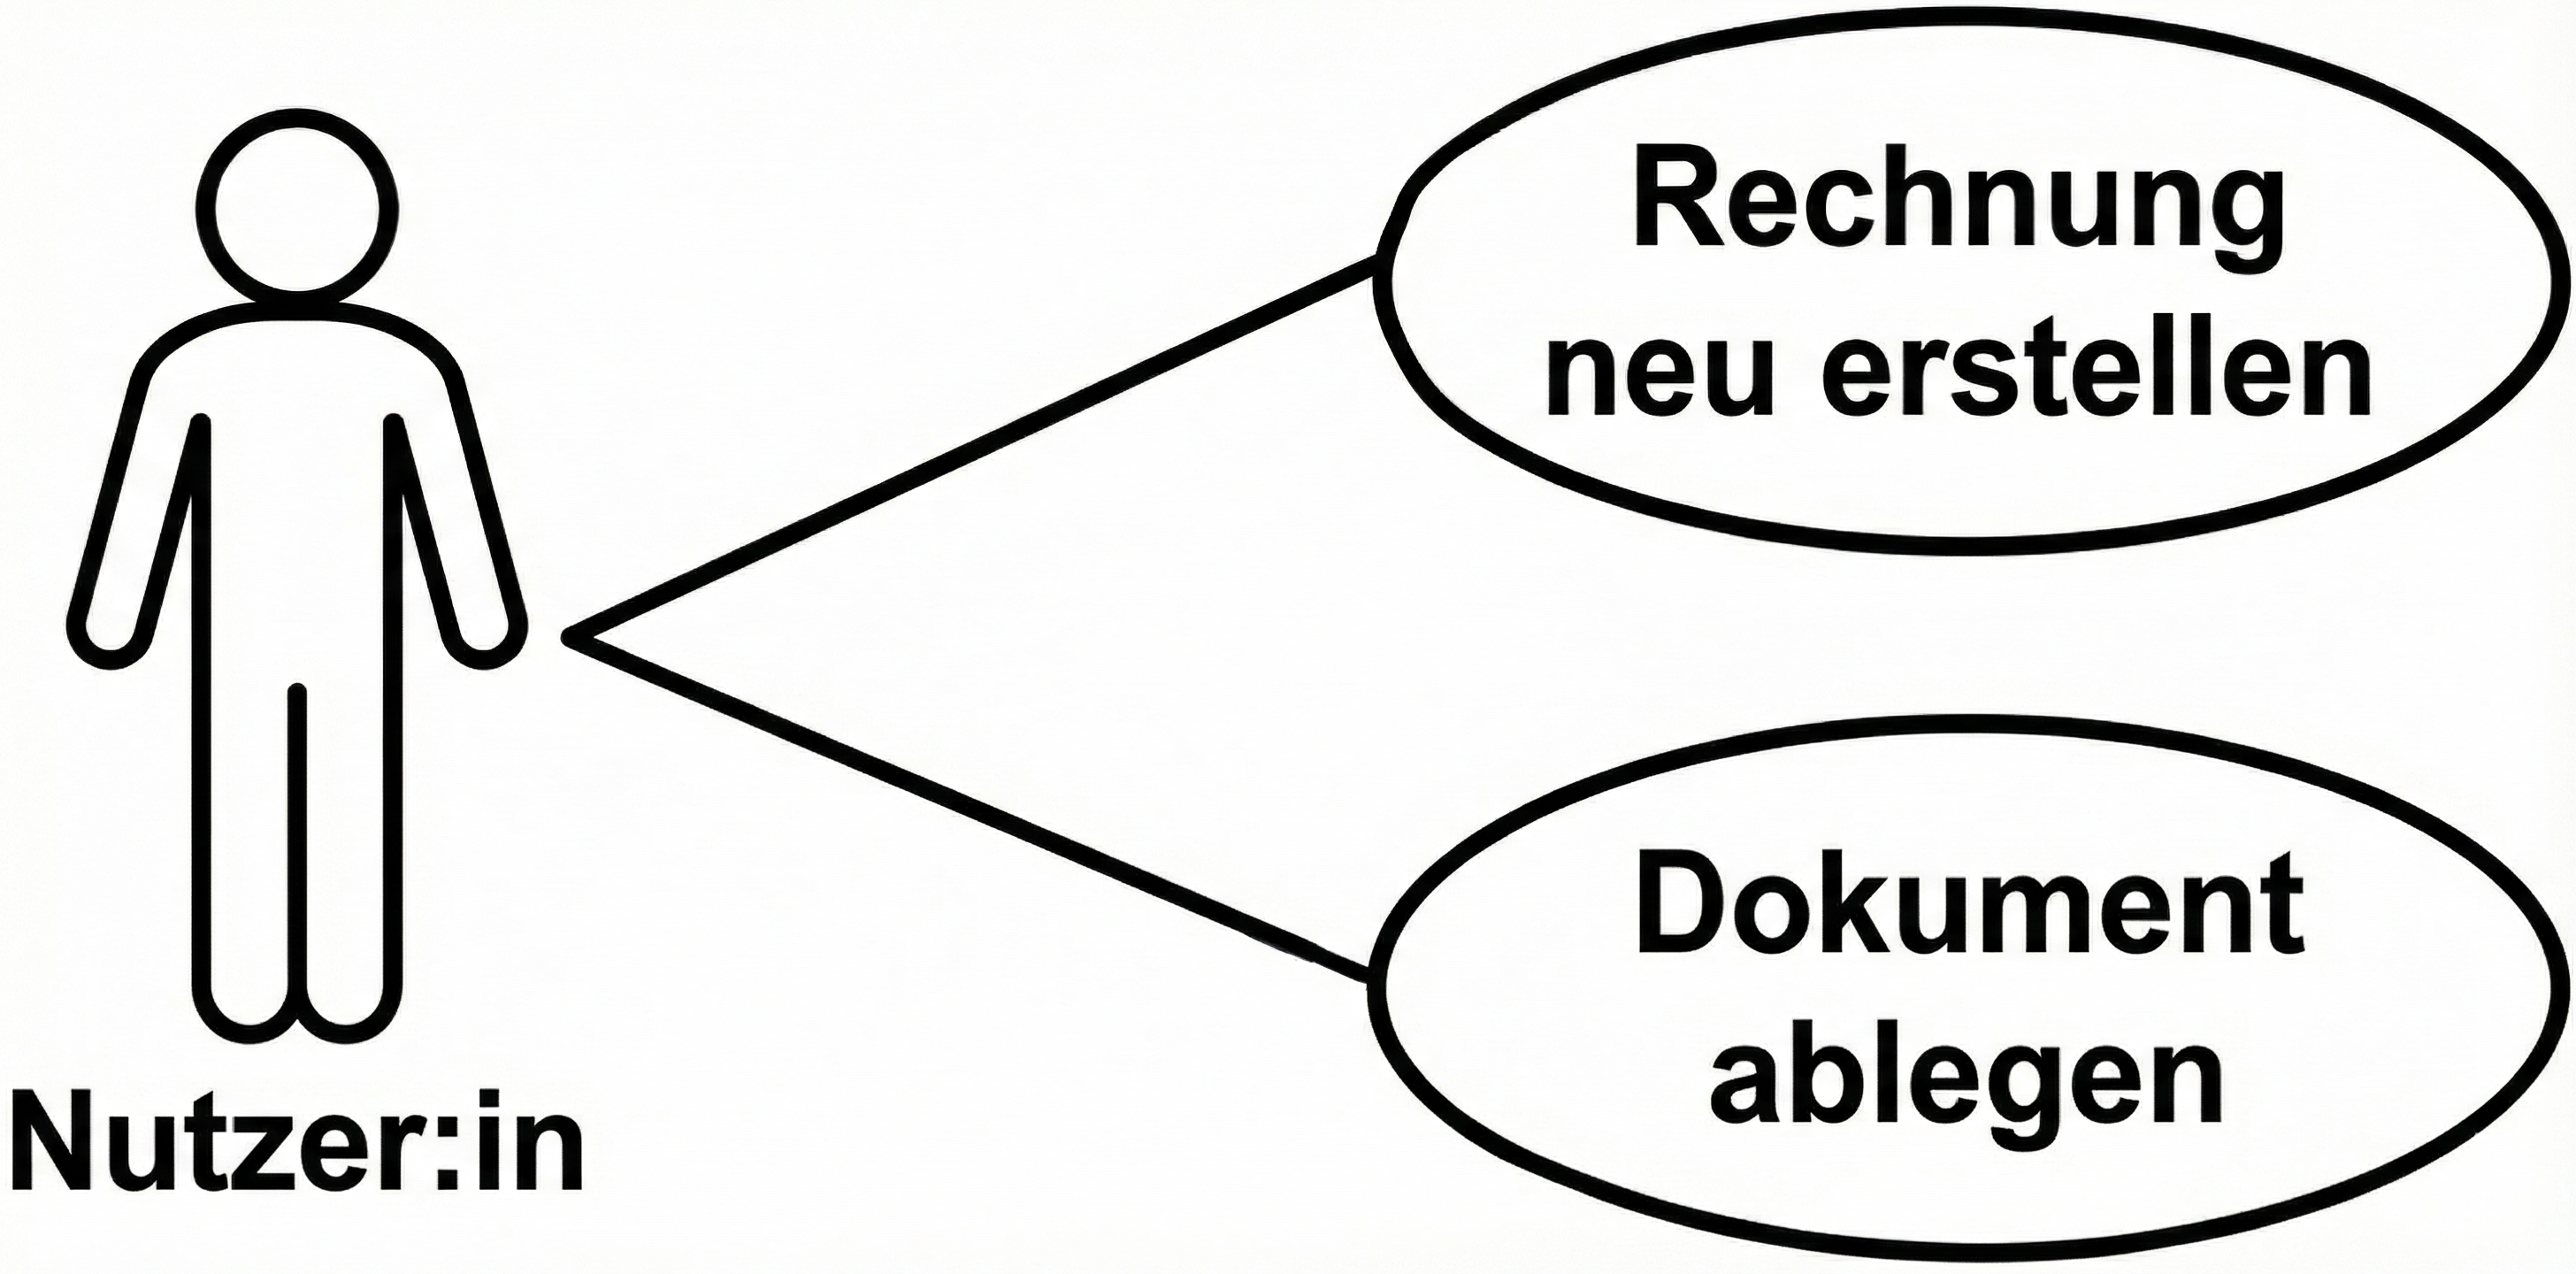
\includegraphics[width=0.8\textwidth]{use_case_diagramm.png}
\caption{Use Cases des Systems: Rechnungserstellung und Dokumentenablage.}
\label{fig:use_cases}
\end{figure}






\section{Zielarchitektur und Systemübersicht}
Die Zielarchitektur des Systems basiert auf mehreren klar abgegrenzten und lose gekoppelten Komponenten, die gemeinsam den End-to-End-Prozess der Rechnungs- und Dokumentenverarbeitung abbilden. Zu den zentralen Elementen zählen der WhatsApp-Chatbot zur Datenerfassung und Prozesssteuerung, Workflows auf der Automatisierungsplattform Make (make.com), eine Airtable-Datenbank als zentrale Datenquelle, Google Docs zur templatebasierten Dokumentenerstellung, Google Drive als Ablagesystem sowie die Web-Anwendung „ClientHub“ für Verwaltung und Zugriff.
Die einzelnen Komponenten sind überwiegend über standardisierte Cloud-\glspl{ac:api} miteinander verbunden. Dadurch können sie unabhängig voneinander betrieben und bei Bedarf flexibel erweitert werden.
\begin{figure}[H]
\centering
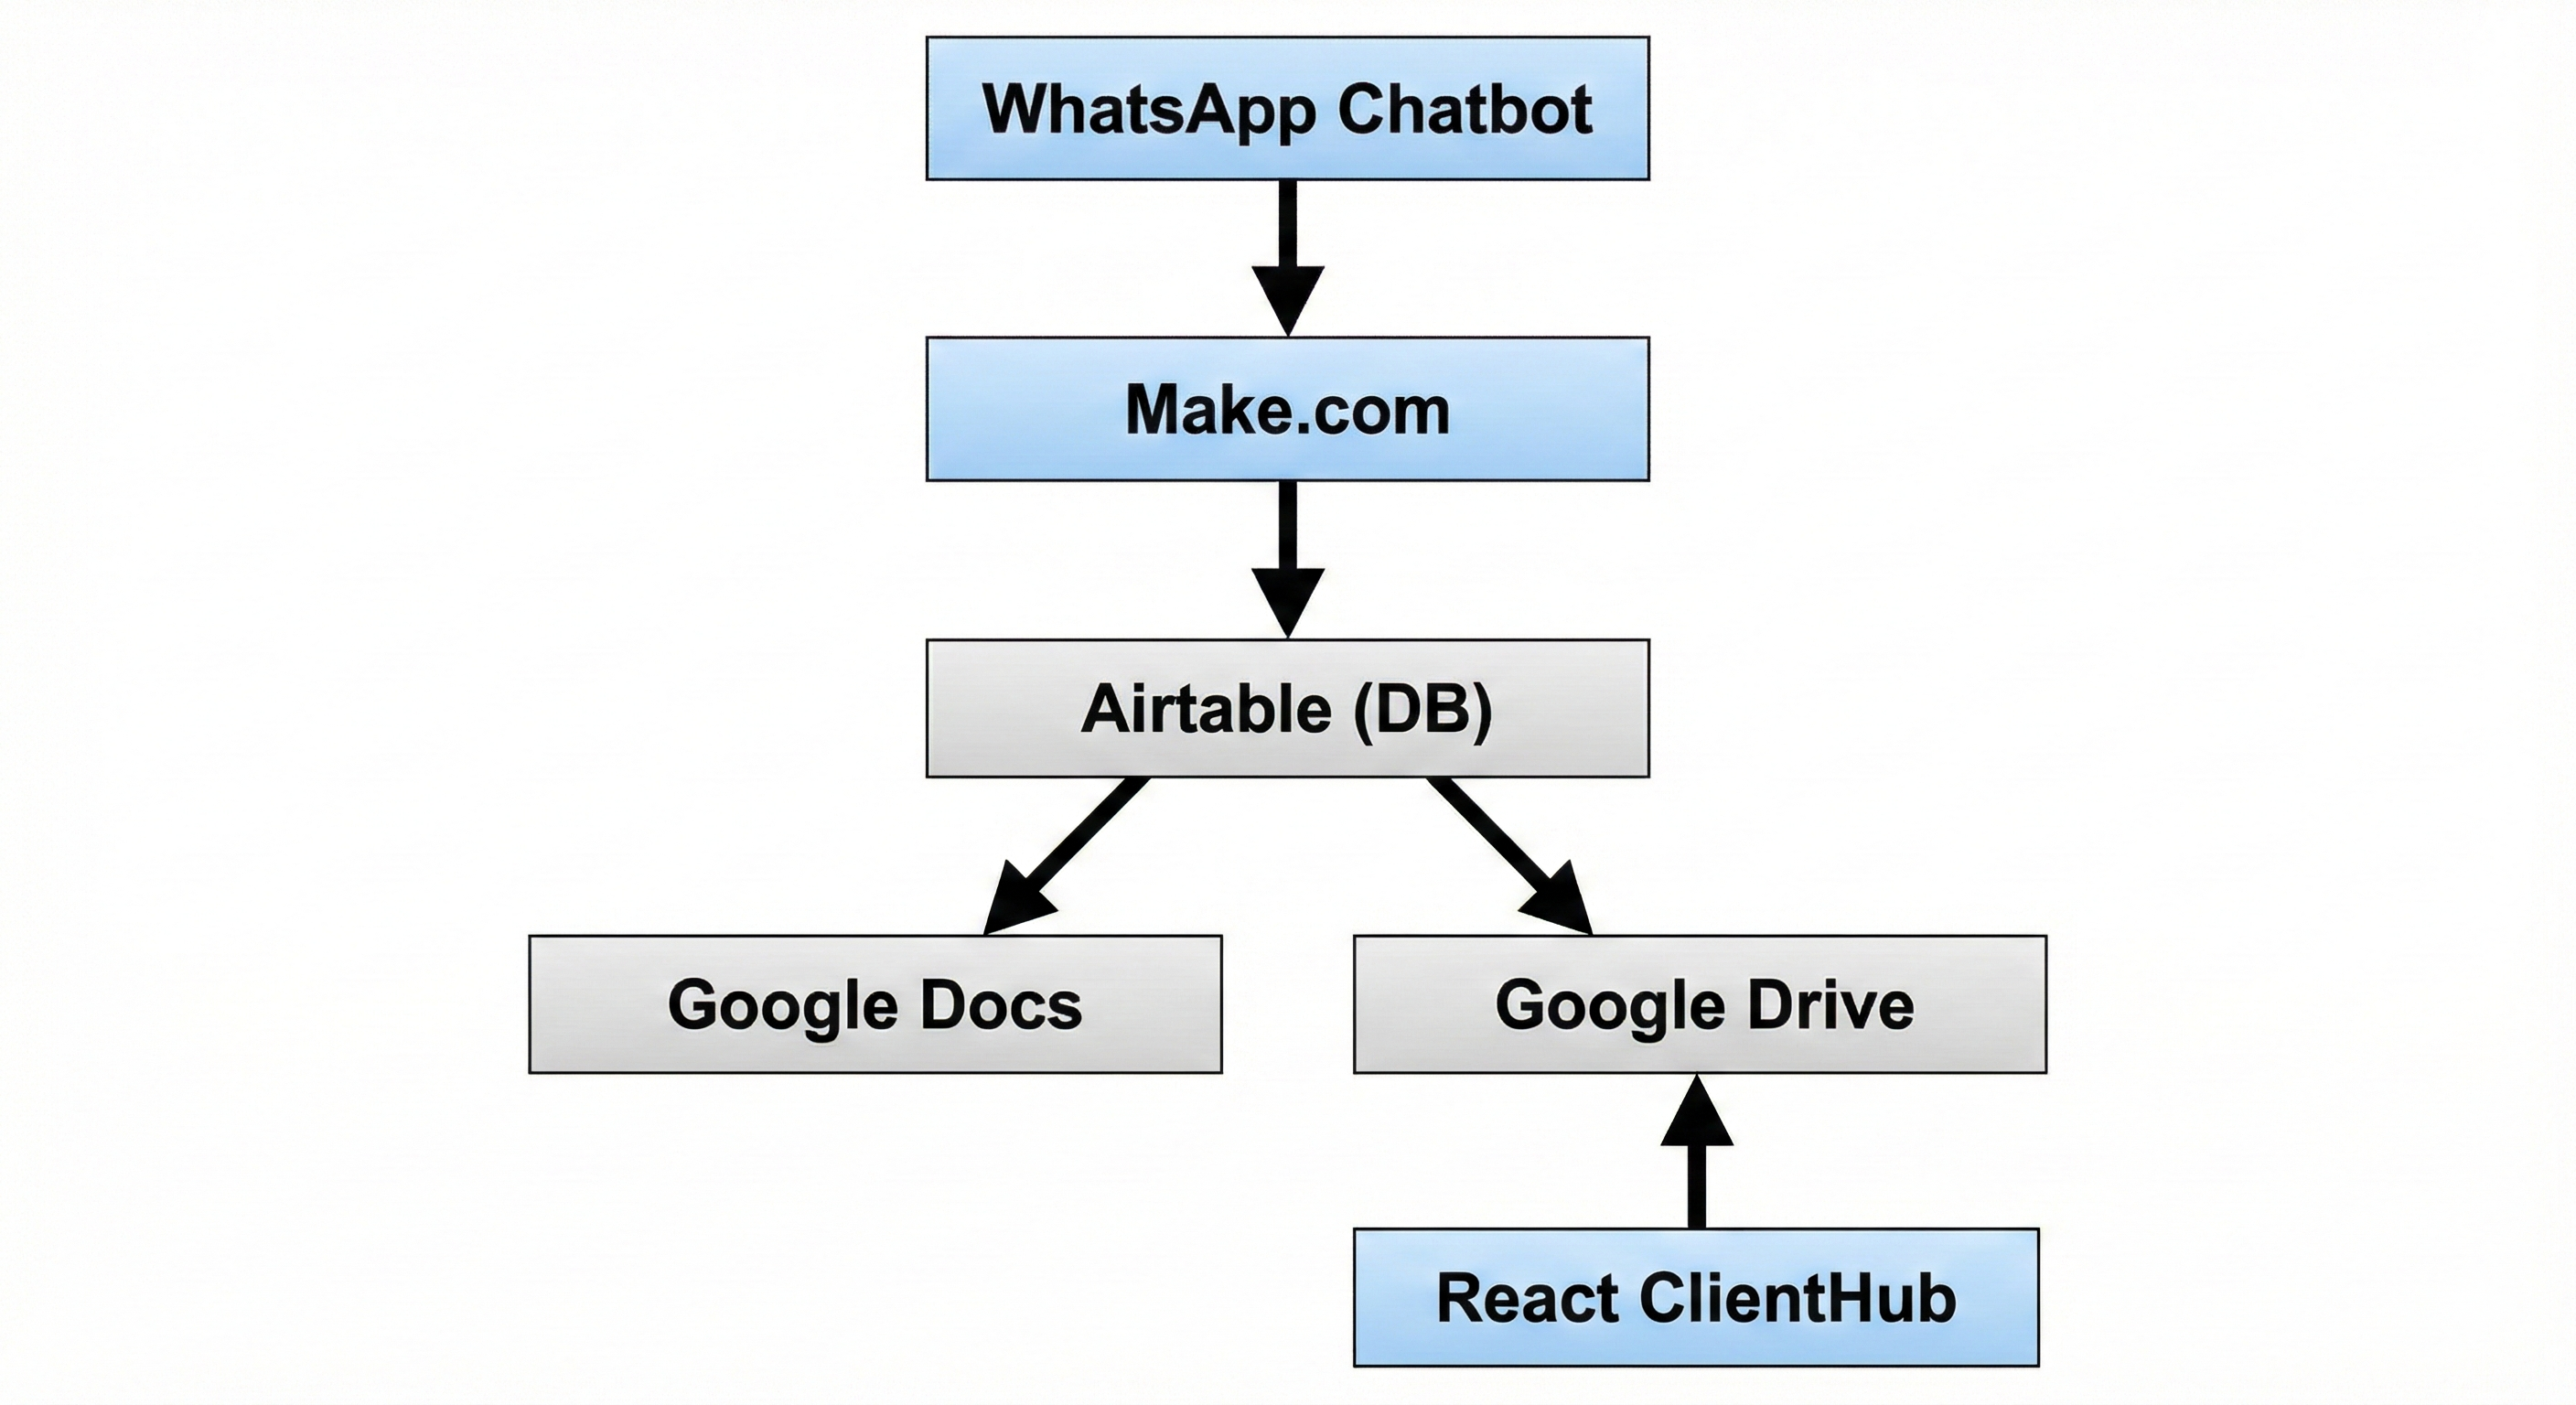
\includegraphics[width=0.9\textwidth]{systemarchitektur.png}
\caption{Zielarchitektur: WhatsApp Chatbot → Make.com → Airtable → Google Docs/Drive → React ClientHub.}
\label{fig:systemarchitektur}
\end{figure}

Das zentrale Element des Systems ist der Chatbot, der über WhatsApp erreichbar ist. Er begleitet die Nutzer dialoggesteuert durch den Prozess der Rechnungsgenerierung, indem er entsprechende Anweisungen gibt. Dies umfasst die Auswahl eines bestehenden Kunden oder die Erstellung eines neuen Kundendatensatzes, die Festlegung der Rechnungspositionen sowie die Bestimmung von Rechnungsnummer, Leistungszeitraum, Zahlungsfrist und Zahlungsart.
Ein weiteres Feature des Chatbots ist die Funktion „Dokument speichern“. Diese erlaubt es den Nutzern, Dateien wie Belege oder bereits erstellte Rechnungen hochzuladen, die anschließend im Kundenportal zur Verfügung gestellt werden. In beiden Szenarien leitet der Chatbot die erfassten Informationen in strukturierter Form an die nachgelagerten Arbeitsabläufe weiter. Er selbst führt keine direkten Abfragen an Datenbank- oder Speicherdiensten durch.

Eine Integrations- und Workflow-Plattform fungiert als Orchestrierungsschicht und implementiert die Logik der Automatisierung. Sie empfängt Nachrichten vom Chatbot, analysiert den aktuellen Dialogschritt und startet kontextabhängig unterschiedliche externe Dienste.
Hierzu zählen insbesondere die Airtable-\gls{ac:api} zur Erstellung und Aktualisierung von Kunden-, Rechnungs- und Sitzungsdaten (z. B. des aktuellen Prozessschritts) \cite{airtable_web_api_guide}, die Google-Docs-\gls{ac:api} zum Öffnen und Befüllen eines vordefinierten Rechnungsmusters sowie die Google-Drive-\gls{ac:api} zur Erstellung von Ordnern und zum Hochladen von Dateien. Ergänzend wird eine KI-Schnittstelle genutzt, um frei formulierte Texte oder Sprachnachrichten in strukturierte, deutschsprachige Rechnungspositionen zu überführen.
Im Rahmen des Dialogs weist der Nutzer die Rechnungsnummer zu. Diese wird als Feld in Airtable gespeichert, um sicherzustellen, dass sie in allen nachfolgenden Prozessschritten konsistent verwendet wird.

Google Drive fungiert als unabhängiges Speichersystem, das insbesondere im Anwendungsfall „Dokument ablegen“ genutzt wird. Der Nutzer startet diesen Vorgang, indem er über den Chatbot eine Datei hochlädt, die durch einen Workflow in eine kundenbezogene Ordnerstruktur überführt wird. Die Verzeichnisse sind nach Jahr, Quartal und Monat gegliedert; ist ein Ordner noch nicht vorhanden, wird er dynamisch erstellt.
Der archivierte Dateilink wird in Airtable gespeichert, sodass er für nachgelagerte Automatisierungen sowie für die Anzeige im Kundenportal verfügbar ist. Auf diese Weise entsteht eine konsistente und nachvollziehbare Archivierung, die sowohl interne Anforderungen als auch die Zusammenarbeit mit Steuerberaterinnen und Steuerberatern unterstützt.

Die Webanwendung „ClientHub“ ist eine browserbasierte React-Anwendung, die als eigenständiges Modul fungiert und ausschließlich serverseitige Edge-Funktionen nutzt, um auf externe Dienste zuzugreifen. Diese Edge-Funktionen bilden die Backend-Schicht der Architektur ab. Sie übernehmen die Interaktion mit der Airtable-\gls{ac:api} und der Google-Drive-\gls{ac:api}, bereiten die Daten für das Frontend auf und schützen gleichzeitig sensible Zugangsdaten vor einem direkten Zugriff aus dem Browser.
Die Webanwendung stellt den Nutzern ein Dashboard mit aggregierten Metriken zur Verfügung. Darüber hinaus bietet sie eine Kundenliste mit Such- und Filteroptionen sowie eine Übersicht über die Ordnerstruktur des Kundenportals, über die archivierte Dokumente eingesehen und heruntergeladen werden können.

Das Design folgt bewusst den architektonischen Grundsätzen der losen Kopplung, der Modularität und der klaren Schichtentrennung. Die Frontend-Logik, die Orchestrierung der Integrationsprozesse und die Datenhaltung sind voneinander entkoppelt. Dadurch können Änderungen in einer Komponente, wie etwa der Austausch des Chatkanals oder die Erweiterung der Datenstruktur, mit nur minimalen Anpassungen in den übrigen Systemteilen umgesetzt werden.
Durch den konsequenten Einsatz von Cloud-Diensten und standardisierten \glspl{ac:api} ist keine eigene Serverinfrastruktur erforderlich. Betrieb, Skalierung und Verfügbarkeit werden größtenteils von den jeweiligen Plattformanbietern übernommen. Die Architektur weist damit Eigenschaften auf, die sie besonders geeignet für kleine Unternehmen machen, die mit begrenzten Ressourcen arbeiten, einen geringen Wartungsaufwand benötigen und dennoch eine Lösung suchen, die flexibel mit wachsenden Anforderungen erweitert werden kann. Lose Kopplung, Modularität und eine klare Schichtentrennung gelten in der Softwarearchitektur als wesentliche Voraussetzungen für wartbare und erweiterbare Systeme. \cite{balzert_softwaretechnik_2011}.
Der konsequente Einsatz wohldefinierter \glspl{ac:api} wird als zentraler Baustein integrationsfähiger, verteilter Systeme beschrieben \cite{spichale_apidesign_2020}.


\section{Datenmodell und Datenflüsse}

Das zugrunde liegende Datenmodell und die zentralen Datenflüsse, die die dialogbasierte Rechnungserstellung sowie die Ablage geschäftsrelevanter Dokumente unterstützen, werden im folgenden Abschnitt erläutert. Die Daten werden in mehreren Airtable-Tabellen gespeichert, die gemeinsam den Chatbot-Dialog, die Rechnungserstellung und die Dokumentenablage in Google Drive abbilden. Die Tabellen dienen dabei nicht nur als persistenter Speicher fachlicher Informationen, sondern bilden zugleich die Grundlage für die Steuerung der Workflows in der Automatisierungsplattform, indem sie Zustandsinformationen und temporäre Eingaben strukturiert bereitstellen.

Im Datenmodell steht die Tabelle „User\_Sessions“ im Mittelpunkt. Sie fungiert als zentrale Instanz zur Verwaltung von Nutzerzuständen und zur Zugriffskontrolle innerhalb des Chatbot-Workflows. In dieser Tabelle werden die Telefonnummern der Nutzer gespeichert, sodass eingehende WhatsApp-Nachrichten validiert und ausschließlich registrierte Rufnummern zum Systemzugang zugelassen werden. Darüber hinaus enthält „User\_Sessions“ Zustandsvariablen wie „Current Step“ und „Next Step“, die zur Steuerung des dialogbasierten Ablaufs verwendet werden. Diese Informationen sind erforderlich, da die eingesetzte Automatisierungsplattform lediglich ein einzelnes Watch-Event für eingehende Nachrichten bereitstellt und keine native Unterstützung für eine zustandsabhängige Dialogführung bietet.
\begin{figure}[H]
\centering
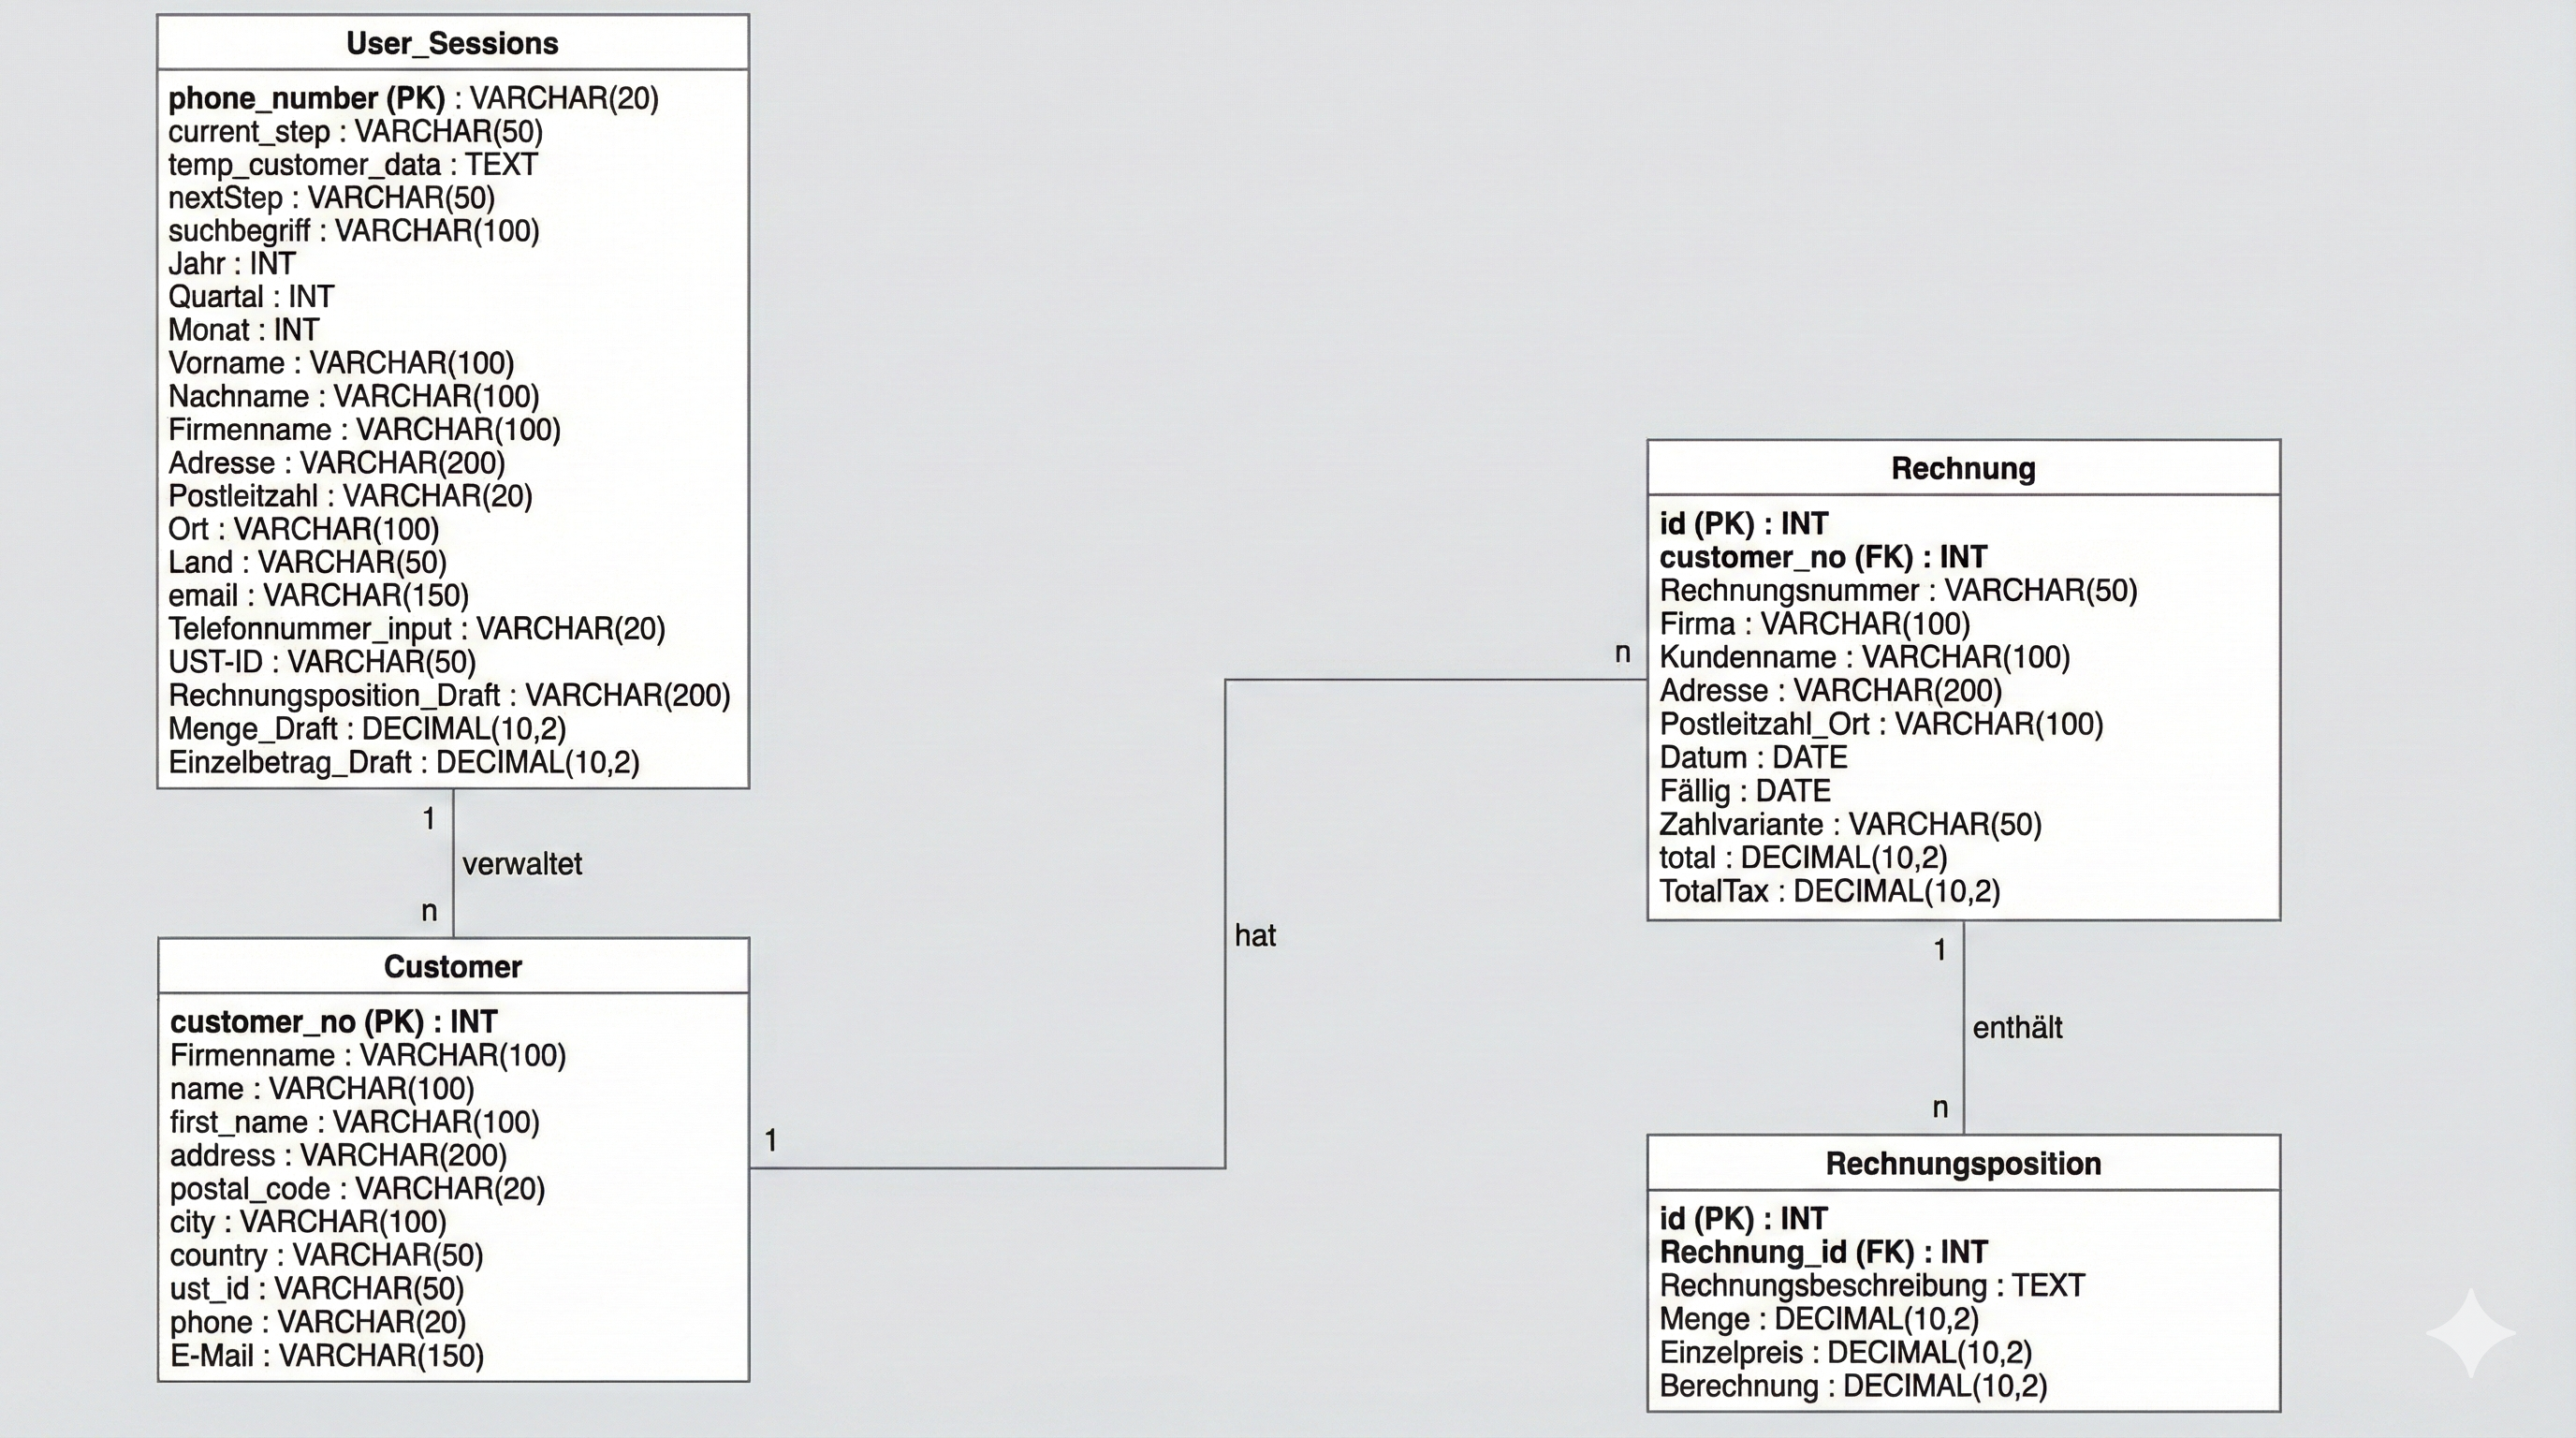
\includegraphics[width=0.9\textwidth]{datenmodell_er.png}
\caption{Airtable-Datenmodell mit Relationen (User\_Sessions, Customer, Rechnung, Rechnungsposition).}
\label{fig:datenmodell}
\end{figure}


„User\_Sessions“ enthält ausschließlich dynamische, während des Gesprächsverlaufs veränderliche Felder. Diese dienen der temporären Speicherung von Nutzereingaben und ermöglichen eine iterative, dialogorientierte Datenerfassung. Ein zentrales Ziel dieser Struktur besteht darin, Korrekturen und Anpassungen durch die Nutzenden jederzeit zuzulassen. Gibt eine Person beispielsweise versehentlich ein falsches Rechnungsjahr an, kann dieser Wert direkt im Chat korrigiert werden. Der entsprechende Eintrag in „User\_Sessions“ wird aktualisiert, und der Workflow setzt mit den korrigierten Daten fort, ohne dass der gesamte Dialog erneut durchlaufen werden muss.

Ein vergleichbares Vorgehen wird bei der Neuanlage von Kunden angewendet. Temporäre Felder wie Vorname, Nachname, Adresse, Postleitzahl und Umsatzsteuer-Identifikationsnummer werden zunächst schrittweise erfasst und können bei Bedarf angepasst werden. Erst nachdem alle erforderlichen Felder vollständig ausgefüllt und eine automatisch generierte Zusammenfassung der Kundendaten explizit bestätigt wurde, erfolgt die dauerhafte Speicherung des Kunden in einer separaten Kundentabelle. Auch rechnungsbezogene Parameter wie Leistungsbeschreibung, Menge und Einzelpreis werden zunächst in „User\_Sessions“ zwischengespeichert. „User\_Sessions“ fungiert somit als transiente Datenspeicherschicht, die keine dauerhafte Persistenz besitzt, sondern ausschließlich der Dialogsteuerung und der Vorbereitung der eigentlichen Geschäftsobjekte dient.

Die dauerhaft gültigen Kundendaten werden in der Tabelle „Customer“ verwaltet, die als zentrale Kundendatenbank des Systems dient. Neue Kundendatensätze können sowohl über die Webanwendung als auch direkt über den Chatbot angelegt werden. In dieser Tabelle werden alle für die Rechnungsstellung relevanten Stammdaten gespeichert, darunter Vor- und Nachname, Firmenbezeichnung, vollständige Adresse, E-Mail-Adresse, Telefonnummer sowie die Umsatzsteuer-Identifikationsnummer. Nach Abschluss eines Neuanlage-Dialogs werden die zuvor in „User\_Sessions“ erfassten temporären Kundendaten in einen konsistenten Datensatz in „Customer“ überführt. Bestehende Kunden werden über ihre in der Tabelle hinterlegten Attribute identifiziert und können im Dialog ausgewählt werden, sodass die bereits gespeicherten Stammdaten ohne erneute Eingabe für die Rechnungserstellung genutzt werden.

Die eigentliche Rechnungslogik ist in den Tabellen „Rechnung“ und „Rechnungsposition“ abgebildet. Die Tabelle „Rechnung“ speichert alle kopfbezogenen Informationen einer Rechnung, insbesondere den zugehörigen Kunden, die Rechnungsnummer, das Rechnungsdatum, den Leistungszeitraum, die Fälligkeit der Forderung sowie die gewählte Zahlungsart. Die hierfür erforderlichen Daten stammen einerseits aus der Tabelle „Customer“, andererseits aus den während des Dialogs in „User\_Sessions“ gespeicherten Eingaben und ergänzenden Feldern, die direkt im Chat erfasst und an Airtable übergeben werden. Zusätzlich werden in „Rechnung“ aggregierte Beträge gespeichert, indem die Summe aller zugehörigen Rechnungspositionen aus der Tabelle „Rechnungsposition“ übernommen und als Grundlage für die Berechnung des Bruttobetrags einschließlich Umsatzsteuer verwendet wird. Diese Berechnungen erfolgen über Formel-Felder, die den Nettobetrag mit einem vordefinierten Steuersatz multiplizieren und auf zwei Nachkommastellen runden.

Die Tabelle „Rechnungsposition“ erfasst die einzelnen Positionen einer Rechnung. Für jede Position werden Daten wie die Leistungsbeschreibung, die Menge und der Einzelpreis gespeichert, die zuvor dialogbasiert erhoben und in „User\_Sessions“ zwischengespeichert wurden. Die Berechnung des Positionsbetrags erfolgt über ein Formel-Feld, indem die Menge mit dem numerischen Einzelpreis multipliziert wird. Da eine Rechnung typischerweise mehrere Positionen umfassen kann, werden für jede Position separate Datensätze angelegt. Die Zuordnung der einzelnen Rechnungspositionen zu einer Rechnung erfolgt über Referenzinformationen wie die Rechnungsnummer oder interne Identifikatoren innerhalb der Workflow-Logik, ohne dass zwingend explizite Verknüpfungsfelder im Airtable-Schema definiert werden müssen.

Der Datenfluss im Anwendungsfall „Rechnung neu erstellen“ beginnt mit dem Eingang einer WhatsApp-Nachricht, mit der der Nutzer den Erstellungsprozess startet. Zunächst wird eine neue Sitzung in „User\_Sessions“ angelegt oder eine bestehende Sitzung aktualisiert, indem die Telefonnummer gespeichert und die Zustandsvariablen initialisiert werden. Anschließend werden alle für die Rechnungserstellung erforderlichen Informationen dialogbasiert erhoben und in den dynamischen Feldern von „User\_Sessions“ zwischengespeichert, darunter Kundendaten, Leistungsbeschreibungen, Mengen, Einzelpreise, Rechnungsdatum, Leistungszeitraum und Zahlungsfrist. Sobald alle Kundendaten vollständig vorliegen und bestätigt wurden, überführt der Workflow die temporären Angaben in einen dauerhaften Datensatz in „Customer“, sofern ein neuer Kunde anzulegen ist. Bei bestehenden Kunden wird lediglich der entsprechende Datensatz referenziert.

Im nächsten Schritt erzeugt der Workflow einen neuen Eintrag in der Tabelle „Rechnung“ und legt parallel für jede erfasste Rechnungsposition einen Datensatz in „Rechnungsposition“ an, der die zuvor zwischengespeicherten Leistungsdaten übernimmt. Nach Abschluss der Positionserfassung werden in „Rechnung“ die relevanten Summen berechnet, indem die Beträge der zugeordneten Positionen aggregiert und um die Umsatzsteuer ergänzt werden. Auf Basis dieser Daten wird in Google Docs ein Rechnungsdokument auf Grundlage eines vordefinierten Templates generiert, das die aus Airtable stammenden Felder einfügt und anschließend über die Google-Drive-\gls{ac:api} als \gls{ac:pdf} exportiert wird \cite{google_docs_api,google_drive_files_export_2025}.
 Das fertige Dokument wird dem Nutzer über den Chat zur Verfügung gestellt und kann für weitere Prozesse, etwa die Ablage oder den Versand, verwendet werden.

Der Datenfluss im Anwendungsfall „Dokument ablegen“ ist ebenfalls dialoggesteuert, fokussiert sich jedoch auf die strukturierte Archivierung von Dateien. Der Prozess wird durch das Hochladen eines Dokuments, beispielsweise eines Belegs oder einer externen Rechnung, über den WhatsApp-Chatbot initiiert. Im Dialog werden die zur Zuordnung notwendigen Informationen erfasst, insbesondere der betroffene Kunde sowie der zeitliche Kontext der Ablage (Jahr, Quartal, Monat), und temporär in einer Sitzung gehalten. Auf Basis dieser Parameter erstellt der Workflow die entsprechende Ordnerstruktur in Google Drive, sofern diese noch nicht existiert, und lädt das Dokument in den kundenbezogenen Unterordner hoch.

Der dabei erzeugte Dateilink steht dem System für nachgelagerte Schritte zur Verfügung, etwa zur Anzeige im Kundenportal. Durch diesen Ablauf wird sichergestellt, dass hochgeladene Dokumente konsistent, nachvollziehbar und eindeutig in Bezug auf Kunde und Zeitraum zugeordnet werden können, ohne dass manuell eine eigene Ablagestruktur gepflegt werden muss.

\section{Prozessablauf vom Chatbot bis zur Ablage}
\subsection{Ablauf „Rechnung neu erstellen“}
In diesem Unterabschnitt wird der Ablauf des Anwendungsfalls „Rechnung neu erstellen“ beschrieben. Der Prozess beginnt mit der Interaktion der Nutzerinnen und Nutzer im WhatsApp-Chat. Anschließend werden die erforderlichen Rechnungsdaten schrittweise erfasst und gespeichert. Auf dieser Grundlage wird ein Rechnungsdokument erstellt, das den Nutzern am Ende des Prozesses als \gls{ac:pdf} direkt im Chat zur Verfügung gestellt wird.

Der Ablauf beginnt, sobald der Nutzer nach der initialen Verifizierung im WhatsApp-Chat den Befehl \glqq Start\grqq{} sendet und im angezeigten Hauptmenü die Option \glqq Rechnung erstellen\grqq{} auswählt. Anschließend wird in der Tabelle \texttt{User\_Sessions} ein Sitzungseintrag angelegt oder aktualisiert. Das Zustandsfeld \texttt{current\_step} wird dabei auf den entsprechenden Wert gesetzt, um den weiteren Dialogverlauf zu steuern.
Auf Basis dieses Sitzungszustands führt der Chatbot den Nutzer schrittweise durch den Prozess. Nach jeder Eingabe wird gezielt die nächste passende Frage gestellt und der aktuelle Zustand entsprechend aktualisiert.


Im ersten inhaltlichen Schritt entscheidet der Nutzer, ob ein neuer Kunde angelegt oder ein bestehender Kunde ausgewählt werden soll. Wird die Option zur Neuanlage gewählt, führt der Chatbot den Nutzer schrittweise durch die Erfassung der erforderlichen Stammdaten.
Dabei wird jedes Datenfeld einzeln abgefragt und zunächst temporär in der Tabelle \texttt{User\_Sessions} gespeichert. Am Beispiel des Vornamens wird dieser Wert nach der Eingabe in einem dynamischen Feld hinterlegt und anschließend durch eine Bestätigungsfrage (\glqq Ist der eingegebene Vorname korrekt?\grqq{}) verifiziert. Abhängig von der Antwort wird entweder der nächste Dialogschritt eingeleitet oder die Eingabe erneut abgefragt.
Dieses Vorgehen wird analog für weitere Stammdaten wie Nachname, Firmenname, Adresse, Postleitzahl, Ort, Land, E\hyp{}Mail\hyp{}Adresse, Telefonnummer sowie die Umsatzsteuer\hyp{}Identifikationsnummer angewendet. Nachdem alle erforderlichen Angaben vollständig erfasst und bestätigt wurden, werden die gesammelten Daten aus \texttt{User\_Sessions} in einen neuen, dauerhaften Datensatz in der Tabelle \texttt{Customer} überführt. Gleichzeitig werden die kopfbezogenen Kundendaten für die spätere Erstellung der Rechnungsvorlage vorbereitet.


Entscheidet sich der Nutzer für die Auswahl eines bestehenden Kunden, wird zunächst ein Suchbegriff abgefragt und in der Tabelle \texttt{User\_Sessions} gespeichert. Auf Grundlage dieses Suchbegriffs werden passende Kundendatensätze ermittelt, woraufhin der Chatbot unterschiedliche Dialogpfade anbietet.
Ergibt die Suche keinen Treffer, kann der Nutzer entweder einen neuen Kunden anlegen, einen weiteren Suchversuch starten oder den Vorgang abbrechen. Führt die Suche zu genau einem Ergebnis, kann dieser Kundendatensatz direkt übernommen oder eine erneute Suche ausgelöst werden. Werden mehrere passende Kunden gefunden, zeigt der Chatbot eine Auswahlliste an, aus der der gewünschte Datensatz ausgewählt werden kann.
In allen Fällen führt eine erfolgreiche Kundenauswahl dazu, dass die entsprechende Kundenreferenz in \texttt{User\_Sessions} hinterlegt wird. Zusätzlich werden die kopfbezogenen Kundendaten in der Tabelle \texttt{Rechnung} gesetzt, um den weiteren Rechnungsprozess vorzubereiten.


An die Kundenauswahl schließt sich die Erfassung der rechnungsbezogenen Daten an. Zunächst wird das Rechnungsdatum abgefragt. Dabei kann der Nutzer entweder das aktuelle Datum (\glqq heute\grqq{}) auswählen oder ein eigenes Datum im Format \texttt{TT.MM.JJJJ} angeben.
Die eingegebene Datumsangabe wird zunächst in \texttt{User\_Sessions} gespeichert und anschließend in das entsprechende Datumsfeld der Tabelle \texttt{Rechnung} übernommen. Im nächsten Schritt wird die Rechnungsnummer im vorgegebenen Format erfasst und ebenfalls dort hinterlegt.
Auf Grundlage dieser Angaben ist der Rechnungskopf vollständig beschrieben. Anschließend beginnt die Erfassung der einzelnen Rechnungspositionen.


Die Erfassung der Rechnungspositionen erfolgt dialogbasiert und unterstützt sowohl Texteingaben als auch Sprachnachrichten. Zunächst wird eine Leistungsbeschreibung abgefragt. Diese kann entweder direkt als Text eingegeben oder aus einer Sprachnachricht transkribiert werden.
Optional kann eine KI\hyp{}Schnittstelle genutzt werden, um aus einer frei formulierten Beschreibung eine prägnante und formal geeignete Rechnungsposition zu erzeugen. Das generierte Ergebnis wird dem Nutzer zur Bestätigung im Chat angezeigt.
Nach der Bestätigung der Leistungsbeschreibung fragt der Chatbot nacheinander die Menge und den Einzelpreis ab. Die eingegebenen Werte werden jeweils temporär in \texttt{User\_Sessions} gespeichert und durch kurze Rückfragen bestätigt. Sobald alle Angaben vollständig vorliegen, werden die Daten in einen neuen Datensatz in der Tabelle \texttt{Rechnungsposition} überführt.
Anschließend kann der Nutzer entscheiden, ob weitere Rechnungspositionen erfasst werden sollen. Wird dies bestätigt, wiederholt sich der beschriebene Ablauf für die nächste Position.


Sind alle Rechnungspositionen erfasst, werden im letzten Schritt die Zahlungsbedingungen abgefragt. Dazu gehört zunächst die Auswahl der Zahlungsfrist, beispielsweise 7, 14 oder 30 Tage. Diese wird im entsprechenden Feld der Tabelle \texttt{Rechnung} gespeichert.
Darüber hinaus wird die gewünschte Zahlart erfasst, etwa Barzahlung, Kartenzahlung oder Überweisung. Auch diese Information wird als weiteres Attribut in der Tabelle \texttt{Rechnung} hinterlegt.
Auf Grundlage der erfassten Daten werden anschließend die relevanten Summen berechnet. Hierzu aggregiert Airtable die Beträge der verknüpften Datensätze aus der Tabelle \texttt{Rechnungsposition} und ergänzt diese um die Umsatzsteuer. Damit liegen alle für die Rechnung erforderlichen Informationen strukturiert in den Tabellen \texttt{Customer}, \texttt{Rechnung} und \texttt{Rechnungsposition} vor.


Auf Basis der in Airtable vorliegenden Daten wird abschließend ein Rechnungsdokument erstellt. Hierzu wird in Google Docs ein vordefiniertes Template geöffnet und mit den Werten aus den Tabellen \texttt{Rechnung}, \texttt{Rechnungsposition} und \texttt{Customer} befüllt. Dabei werden die im Dokument enthaltenen Platzhalter durch die entsprechenden Feldinhalte ersetzt.
Das fertig befüllte Dokument wird anschließend als \gls{ac:pdf} bereitgestellt. Zum Abschluss erhält der Nutzer im WhatsApp\hyp{}Chat die fertige Rechnung in Form einer \gls{ac:pdf}\hyp{}Datei.
Damit ist der gesamte Prozess von der initialen Interaktion im Chat bis zur Bereitstellung des formalen Rechnungsdokuments vollständig automatisiert abgeschlossen.

\subsection{Ablauf „Dokument ablegen“}
Der Anwendungsfall \glqq Dokument ablegen\grqq{} beschreibt den dialogbasierten Ablauf, mit dem Nutzerinnen und Nutzer Belege oder andere geschäftsrelevante Dokumente über den WhatsApp-Chat hochladen können. Ziel dieses Prozesses ist die strukturierte Ablage der Dokumente, sodass sie später zuverlässig wiedergefunden werden können.
Ähnlich wie beim Anwendungsfall zur Rechnungserstellung erfolgt der Einstieg über den Chatbot. Die weitere Verarbeitung der Daten sowie die Ablage der Dokumente werden durch die angebundenen Systeme im Hintergrund gesteuert.


Der Ablauf beginnt, sobald die Nutzerin oder der Nutzer den Chat mit dem Rechnungsbot öffnet und nach der initialen Verifizierung den Befehl \glqq Start\grqq{} sendet. Daraufhin zeigt der Chatbot ein Hauptmenü mit den Optionen \glqq Rechnung erstellen\grqq{} und \glqq Dokument speichern\grqq{} an.
Wählt der Nutzer die Option \glqq Dokument speichern\grqq{}, wird in der Tabelle \texttt{User\_Sessions} ein entsprechender Sitzungseintrag angelegt oder aktualisiert. Gleichzeitig wird das Zustandsfeld \texttt{current\_step} so gesetzt, dass der folgende Dialog eindeutig dem Anwendungsfall \glqq Dokument ablegen\grqq{} zugeordnet ist.


Im ersten Schritt der Dokumentenablage wird der zeitliche Kontext für die spätere Ablagestruktur festgelegt. Dazu fordert der Chatbot die Nutzerinnen und Nutzer auf, ein Jahr auszuwählen. In der Regel stehen dabei das aktuelle Jahr sowie die beiden unmittelbar vorangegangenen Jahre zur Auswahl, beispielsweise 2023, 2024 und 2025.
Die getroffene Auswahl wird in der Tabelle \texttt{User\_Sessions} in einem entsprechenden Feld, etwa \texttt{Jahr}, gespeichert. Gibt die Nutzerin oder der Nutzer eine ungültige Eingabe ein, die erneute Auswahl des Jahres angefordert.
Dieses Vorgehen stellt sicher, dass für die spätere Ordnerbildung ausschließlich zulässige Werte verwendet werden.


Nachdem das Jahr erfolgreich festgelegt wurde, fragt der Chatbot im nächsten Schritt das zugehörige Quartal ab. Hierzu werden die vier Quartale des Jahres in einer Auswahlliste angezeigt. Die getroffene Auswahl wird in der Tabelle \texttt{User\_Sessions}, beispielsweise im Feld \texttt{Quartal}, gespeichert.
Anschließend wird der Monat abgefragt, der innerhalb des zuvor gewählten Quartals liegt. Dabei ist die Auswahl auf die Monate des entsprechenden Quartals beschränkt. Auf diese Weise können die Nutzerinnen und Nutzer nur konsistente Kombinationen aus Jahr, Quartal und Monat angeben.
Eingaben, die nicht der vorgegebenen Auswahl entsprechen, werden zurückgewiesen und führen zu einer erneuten Abfrage.


Sobald Jahr, Quartal und Monat ausgewählt wurden, liegen alle erforderlichen Metadaten für die spätere Ablagestruktur vor. Diese Informationen werden in der Tabelle \texttt{User\_Sessions} gespeichert. Gleichzeitig wird der Zustandsparameter \texttt{current\_step} auf den nächsten Verarbeitungsschritt gesetzt, der den Uploadvorgang einleitet.
Anschließend fordert der Chatbot die Nutzerinnen und Nutzer dazu auf, das zu archivierende Dokument direkt im WhatsApp-Chat hochzuladen \cite{whatsapp_cloud_api_media_2025}. Dabei kann es sich beispielsweise um eine externe Rechnung, einen Zahlungsbeleg oder ein anderes geschäftsrelevantes Dokument handeln.


Geht ein Dokument im Chat ein, wird die Datei vom Workflow entgegengenommen und der erfolgreiche Upload gegenüber der Nutzerin oder dem Nutzer bestätigt. Anschließend prüft das System, ob die erforderliche Ordnerstruktur in Google Drive bereits vorhanden ist.
Die Ablage erfolgt in einer hierarchisch aufgebauten Struktur, die sich beispielsweise nach Kunde, Jahr, Quartal und Monat gliedert. Existiert ein Ordner für das ausgewählte Jahr bereits, wird dieser wiederverwendet. Andernfalls wird er neu angelegt. Gleiches gilt für die untergeordneten Ordner auf Quartals- und Monatsebene.
Das hochgeladene Dokument wird abschließend im passenden Monatsordner des zuvor gewählten Jahres und Quartals gespeichert.


Durch diesen Ablauf wird das Dokument konsistent und nachvollziehbar in der vorgesehenen Ablagestruktur archiviert. Die in \texttt{User\_Sessions} erfassten Parameter bilden gemeinsam mit der dynamischen Ordnererstellung in Google Drive die Grundlage für eine eindeutige zeitliche Zuordnung der Dokumente. Dadurch entfällt für die Nutzerinnen und Nutzer die manuelle Pflege von Verzeichnissen oder das Wissen über konkrete Dateipfade.
Dies erleichtert sowohl das spätere Wiederfinden der Dokumente als auch die Nutzung der Ablage für nachgelagerte Prozesse. Dazu zählen beispielsweise die Zusammenarbeit mit Steuerberatungen oder interne Auswertungen.




\section{Sicherheits- und Datenschutzkonzept}